\documentclass[12pt]{article}

\usepackage{fullpage} % Package to use full page
\usepackage{parskip} % Package to tweak paragraph skipping
\usepackage{tikz} % Package for drawing
\usepackage{amsmath}
\usepackage{amsfonts}
\usepackage{dutchcal}
\usepackage{hyperref}
\usepackage{minted}
\usepackage{pythonhighlight}
\usepackage{cite}
\usepackage{bm}
\usepackage{minted}
\usepackage{pythonhighlight}

\usepackage{caption}
%\usepackage[dvipsnames]{xcolor} % 更全的色系

\usepackage{fontspec}
\setmainfont{Times New Roman}
%\setmainfont{Arial}
%\setmainfont{TeX Gyre Termes}

\bibliographystyle{plain}

\title{The Project of DSA5206: Advanced Topics in Data Science}
\author{Huang Rui}
\date{\today}

\begin{document}

\maketitle

\section*{Part1}
\subsection*{(a)}
When $x(t)=0$, the system equation $(1.1)$ simplifies to a homogeneous linear system:
\[
\frac{d}{dt}
\begin{pmatrix}
h_1(t) \\
h_2(t)
\end{pmatrix}
=
\begin{pmatrix}
-1 & 0 \\
0 & -10
\end{pmatrix}
\begin{pmatrix}
h_1(t) \\
h_2(t)
\end{pmatrix}
\]
The leading dynamic mode of the system is determined by the eigenvalues and eigenvectors of the system matrix. The matrix is diagonal, so the dynamic modes correspond to the eigenvalues and eigenvectors of this matrix, which are readily identifiable from the matrix itself. The system matrix has eigenvalues $-1$ and $-10$, with corresponding eigenvectors $[1,0]^T$ and $[0,1]^T$.\\

Since Dynamic Mode Decomposition (DMD) identifies modes associated with dominant behaviors, the leading dynamic mode in this case corresponds to the eigenvalue with the smallest magnitude in absolute terms (less negative), which is $-1$. The corresponding eigenvector is $[1,0]^T$. This vector $[1,0]$ in $ \mathbb{R}^2 $ represents the leading dynamic mode.\\

\subsection*{(b)}
The following code is to discretize the system dynamics, simulate the trajectories, and compute the leading spatial POD mode.
\begin{minted}{python}
# Constants and parameters for simulation
dt = 1e-3  # Time step
total_time = 1  # Total time of simulation
num_steps = int(total_time / dt)  # Number of time steps
num_trajectories = 1000  # Number of trajectories

# Initial conditions
h_initial = np.zeros((2, 1))

# Discrete-time system matrix
A_discrete = np.eye(2) + A * dt
B_discrete = np.array([[1e-3], [1e3]]) * dt

# To store all trajectories
all_trajectories = np.zeros((2, num_steps, num_trajectories))

# Simulate the system
np.random.seed(42)  # for reproducibility
for j in range(num_trajectories):
    h = h_initial.copy()
    for i in range(num_steps):
        x_t = np.random.normal(0, 1)  # Sample x(t)
        h = A_discrete @ h + B_discrete * x_t  # Euler integration step
        all_trajectories[:, i, j] = h.squeeze()

# Perform POD via time-averaging across all trajectories
# Flatten trajectories into a matrix of 2 x (num_steps*num_trajectories)
data_matrix = all_trajectories.reshape(2, -1)  
covariance_matrix = np.cov(data_matrix)  # Compute the covariance matrix
# Eigen-decomposition
pod_eigenvalues, pod_eigenvectors = np.linalg.eig(covariance_matrix)  

# Sort eigenvectors based on eigenvalues in descending order
sorted_indices = np.argsort(-pod_eigenvalues)
leading_pod_mode = pod_eigenvectors[:, sorted_indices[0]]

print(pod_eigenvalues, pod_eigenvectors, leading_pod_mode)
\end{minted}
After simulating the system and performing Proper Orthogonal Decomposition (POD) on the generated dataset, we found the leading spatial POD mode to be approximately $[-1.763 \times 10^{-6},-1]$. This vector represents the direction along which the variance of the data is maximized, hence it's the dominant spatial structure in the data set.

\subsection*{(c)}
For Dynamic Mode Decomposition (DMD): \\
The leading DMD mode we found was $[1,0]$, associated with the system's slower decay rate (eigenvalue $-1$). This mode essentially captures the dynamics of $h_1(t)$ independent of $h_2(t)$. Using this for dimensionality reduction would imply focusing solely on the $h_1(t)$ component while ignoring $h_2(t)$.\\

For Proper Orthogonal Decomposition (POD): \\
The leading POD mode is $[-1.763 \times 10^{-6},-1]$ , which suggests that $h_2(t)$ has much greater variability and is more influential in the dataset generated. Reducing the system to this mode would focus primarily on $h_2(t)$ dynamics, which are more sensitive to the input $x(t)$ due to the large coefficient in $B$.\\

In conclusion, Using the leading DMD mode for reduction might ignore significant input-driven dynamics present in $h_2(t)$. On the other hand, using the leading POD mode captures more of the input effect but might miss simpler decay behaviors of $h_1(t)$. \\
Hence, the choice depends on the specific goals of the analysis or control task: whether we prioritize capturing the most energy variance (POD) or focusing on specific dynamic features (DMD).

\subsection*{(d)}
The state-transition matrix for a linear time-invariant (LTI) system is given by $e^{At}$, which is the matrix exponential of $A$. The solution to the state equation at time $t$, assuming zero initial conditions for simplicity, is given by:
\[
h(t) = \int_{0}^{t} e^{A(t-\tau)} Bx(\tau) \, d\tau
\]
To prove controllability, we need to show that it is possible to transfer the state $h(t)$ from the origin to any final state $h_f$ in finite time using an appropriate control input $x(t)$.\\

For a given time interval $[0,T]$, the controllability Gramian is defined as:
\[
W_c(T) = \int_{0}^{T} e^{A\tau} BB^T e^{A^T\tau} \, d\tau
\]
If $W_c(T)$ is invertible (has full rank), then the system is controllable on $[0,T]$.\\

The columns of the controllability matrix $R$ span the same space as the columns of $W_c(T)$ as $T\rightarrow \infty$. This is because the higher powers of $A$ in the expansion of the matrix exponential $e^{A\tau}$ will span the same subspace as the lower powers of $A$ due to the Cayley-Hamilton theorem, which states that $A_k$ for $k\geq m$ can be expressed as a linear combination of $I,A,A^2,\dots,A^{m-1}$.\\

If $R$ has full rank, this implies that the states that can be reached from the origin within infinite time span the entire state space $\mathbb{R}^m$. Specifically, any state $h_f$ can be written as a linear combination of the columns of $R$, meaning there exists a control sequence $x(t)$ that will transfer the state $h(0)$ to $h_f$ in finite time.\\

Thus, if the controllability matrix $R$ has full column rank $m$, then for any $h_f \in \mathbb{R}^m$, there exists a control input $x(t)$ such that:
\[
h_f = \int_{0}^{T} e^{A(T-\tau)} Bx(\tau) \, d\tau
\]
This concludes that the system is controllable on $[0,T]$ for any $T>0$, and by extension, for any finite time interval.

\subsection*{(e)}
To prove $W_c(t)$ is \textbf{symmetric}:\\
By the properties of the transpose operation and the fact that the matrix exponential is always defined, we have:
\[
\left( e^{A\tau} BB^T e^{A^T\tau} \right)^T = \left( e^{A^T\tau} \right)^T (BB^T)^T \left( e^{A\tau} \right)^T = e^{A\tau} BB^T e^{A^T\tau}
\]
which shows that the integrand is symmetric for each $\tau$ since $(BB^T)^T=BB^T$. Since the integral of symmetric matrices is also symmetric, $W_c(t)$ is symmetric.\\

To prove $W_c(t)$ is \textbf{positive definite}:\\
We need to show that for any non-zero vector $z \in \mathbb{R}^m$, the following condition holds:
\[
z^TW_c(t)z>0
\]
Let's evaluate the quadratic form $z^TW_c(t)z$:
\[
z^T W_c(t) z = \int_{0}^{t} z^T e^{A\tau} BB^T e^{A^T\tau} z \, d\tau
\]
Let $ $, so $ $, and we can rewrite the integral as:
\[
\int_{0}^{t} v(\tau)^T BB^T v(\tau) \, d\tau
\]
Now, $BB^T$ is positive semi-definite (as it is a Gram matrix). Therefore, $v(\tau)^TBB^Tv(\tau)\geq 0$ for all $\tau$. Since $z \neq 0$ and assuming that $R$ has full column rank $m$, there is always some $\tau$ for which $v(\tau)\neq 0$ (since $e^{A\tau}$ is invertible and does not map any non-zero vector to the zero vector). This implies that the integrand is strictly positive for some $\tau$ in the range $[0,t]$, and therefore the integral is strictly positive:
\[
z^TW_c(t)z>0
\]
Hence, $W_c(t)$ is positive definite for any non-zero $z$ and for any $t>0$.

\subsection*{(f)}
We need to show that with the input $x_*(t)$, the state $h(t_*)$ will be equal to $h_\star$.\\
Given the control input \( x_*(t) \), let's compute the state \( h(t) \) at time \( t = t_* \), using the state-transition equation:
\[
h(t) = e^{A t} h(0) + \int_{0}^{t} e^{A(t-\tau)} Bx(\tau) \, d\tau
\]
Since we want the system to start at the origin, let's set \( h(0) = 0 \), which simplifies the equation to:
\[
h(t) = \int_{0}^{t} e^{A(t-\tau)} Bx(\tau) \, d\tau
\]
Now we substitute \( x(\tau) \) with \( x_*(\tau) \):
\[
h(t) = \int_{0}^{t} e^{A(t-\tau)} BB^T e^{A^T(t_*-\tau)} W_c(t_*)^{-1} h_*(\tau) \, d\tau
\]
Let's change the variable of integration from \( \tau \) to \( \sigma = t_* - \tau \), which changes \( d\tau \) to \( -d\sigma \):
\[
h(t) = - \int_{t_*}^{t_*-t} e^{A(t_*-\sigma)} BB^T e^{A^T\sigma} W_c(t_*)^{-1} h_*(\sigma) \, d\sigma
\]
As \( t \) approaches \( t_* \), the limits of the integral become \( t_* \) to 0, and we take the negative sign into account:
\[
h(t_*) = \int_{0}^{t_*} e^{A(t_*-\sigma)} BB^T e^{A^T\sigma} W_c(t_*)^{-1} h_*(\sigma) \, d\sigma
\]
The integral we have now is the definition of the controllability Gramian at \( t_* \):
\[
h(t_*) = W_c(t_*) W_c(t_*)^{-1} h_*
\]
Thus, we have shown that the state at time \( t_* \) is the desired final state \( h_* \), assuming that the control input \( x_*(t) \) is applied.

\subsection*{(g)}
The energy \( E \) of the input is the integral of the square of the Euclidean norm of \( x_*(s) \) over the interval from \( 0 \) to \( t_* \):
\[
E = \int_{0}^{t_*} | x_*(s) |^2 \, ds = \int_{0}^{t_*} x_*(s)^T x_*(s) \, ds
\]
Substitute \( x_*(s) \) with its definition:
\[
E = \int_{0}^{t_*} (B^T e^{A^T(t_*-s)} W_c(t_*)^{-1} h_k)^T (B^T e^{A^T(t_*-s)} W_c(t_*)^{-1} h_k) \, ds
\]
Then:
\[
E = \int_{0}^{t_*} h_k^T (W_c(t_*)^{-1})^T e^{A(t_*-s)} BB^T e^{A^T(t_*-s)} W_c(t_*)^{-1} h_k \, ds
\]
Since \( W_c(t_*) \) is symmetric, \( (W_c(t_*)^{-1})^T = W_c(t_*)^{-1} \), and we can simplify further:
\[
E = h_k^T W_c(t_*)^{-1} \left( \int_{0}^{t_*} e^{A(t_*-s)} BB^T e^{A^T(t_*-s)} \, ds \right) W_c(t_*)^{-1} h_k
\]
Recognizing the expression within the integral as the definition of the controllability Gramian \( W_c(t_*) \):
\[
E = h_k^T W_c(t_*)^{-1} W_c(t_*) W_c(t_*)^{-1} h_k
\]
Therefore:
\[
E = h_k^T W_c(t_*) h_k
\]
This shows that the energy \( E \) needed to transfer the state from \( 0 \) to \( h_k \) in time \( t_* \) using the control input \( x_*(t) \) is \( h_k^T W_c(t_*) h_k \).

\subsection*{(h)}
the controllability Gramian $W_c(t)$ for the system at time $t=1$ is given by the integral:
\[
W_c(t) = \int_{0}^{t} e^{A\tau} BB^T e^{A^T\tau} \, d\tau
\]
To compute $W_c(1)$ numerically, we can discretize the integral and sum up the contributions from each time step. After we compute $W_c(1)$, we can calculate its eigenvalues.\\
The following is the code for computing:\\
\begin{minted}{python}
import numpy as np
from scipy.linalg import expm, eigvals

# Define the system matrices
A = np.array([[-1, 0],
              [0, -10]])
B = np.array([[1e-3],
              [1e3]])

# Time at which to compute the Gramian
t = 1

# Discretization parameters
num_steps = 1000
delta_t = t / num_steps
Wc = np.zeros((2, 2))

for step in range(num_steps):
    tau = step * delta_t
    Wc += expm(A * tau) @ B @ B.T @ expm(A.T * tau) * delta_t

# Compute the eigenvalues of the controllability Gramian
eigenvalues = eigvals(Wc)

print(Wc)
print(eigenvalues)
\end{minted}
The controllability Gramian $W_c(t)$ for the system at time $t=1$ is approximately:
\[
W_c(1) \approx \begin{pmatrix}
4.32764835 \times 10^{-7} & 9.14084809 \times 10^{-2} \\
9.14084809 \times 10^{-2} & 5.05016666 \times 10^{4}
\end{pmatrix}
\]
And the eigenvalues of the controllability Gramian are approximately:
\[
\begin{split}
\lambda_1 \approx&2.67311407 \times 10^{-7} \\
\lambda_2 \approx&5.05016666 \times 10^4    
\end{split}
\]

\subsection*{(i)}
With the transformation, we can first compute the $\Tilde{A}$ and $\Tilde{B}$. After that, use the new $\Tilde{A}$ and $\Tilde{B}$ to compute $\Tilde{W}_c(1)$.\\
Here is the code for computing:
\begin{minted}{python}
# Define the transformation matrix T
T = np.array([[1e3, 0],
              [0, 1e-3]])

# Compute the new A and B matrices for the transformed system
A_tilde = T @ A @ np.linalg.inv(T)
B_tilde = T @ B

# Compute the controllability Gramian for the transformed system
Wc_tilde = np.zeros((2, 2))

for step in range(num_steps):
    tau = step * delta_t
    Wc_tilde += expm(A_tilde * tau) @ B_tilde @ B_tilde.T 
                @ expm(A_tilde.T * tau) * delta_t

# Compute the eigenvalues of the controllability Gramian
eigenvalues_tilde = eigvals(Wc_tilde)

Wc_tilde, eigenvalues_tilde
\end{minted}
The controllability Gramian $\Tilde{W}_c(t)$ for the system at time $t=1$ is approximately:
\[
\Tilde{W}_c(1) \approx \begin{pmatrix}
0.43276483 & 0.09140848 \\
0.09140848 & 0.05050167
\end{pmatrix}
\]
And the eigenvalues of the controllability Gramian are approximately:
\[
\begin{split}
\Tilde{\lambda}_1 \approx& 0.45349829 \\
\Tilde{\lambda}_2 \approx& 0.02976822  
\end{split}
\]
Observation:\\
\textbf{Gramian Symmetry}: The Gramian remains symmetric, which is consistent with the theory since the Gramian should always be symmetric due to the properties of the state-transition matrix $e^{At}$ and the input matrix $B$.\\

\textbf{Value of controllability Gramian}: The transformed Gramian $\Tilde{W}_c(1)$ occurs to be the $TW_c(1)T^T$, whcih is the same as the transformation of the matrix $A$.\\

\textbf{Impact of Transformation}: The transformation does not change the system's controllability. Controllability is an invariant property under a change of basis (which is what the transformation $T$ is doing). However, the magnitudes of the eigenvalues can change, which influences the "energy" needed to control the system in the new basis.\\

\textbf{Scale of the System}: The transformation $T$ has significantly rescaled the state-space. This changes the numerical values of the Gramian and can change the difficulty of controlling the system due to numerical properties like conditioning.


\newpage
\section*{Part2}
\subsection*{1.Introduction}
About the problem:\\
In the evolving landscape of economic forecasting, the ability to accurately predict commodity prices is paramount for businesses, consumers, and policymakers. This report focuses on forecasting the prices of tortillas across various states in Mexico, a staple food item with significant economic and cultural importance. The goal is to develop a predictive model that provides reliable price forecasts, helping stakeholders make informed decisions in planning, budgeting, and policy-making.\cite{syerramilli2023}\\

About the dataset:\\
The dataset used in this analysis comprises monthly records of tortilla prices per kilogram across different states in Mexico, spanning several years. Each entry in the dataset includes three key pieces of information:
\begin{itemize}
\item \textbf{State:} The Mexican state where the price was recorded.
\item \textbf{Year-Month:} The year and month when the price was recorded, providing a temporal dimension to the dataset.
\item \textbf{Price per Kilogram:} The price of tortillas per kilogram in Mexican pesos, serving as the target variable for our forecasts.
\end{itemize}

\subsection*{2.Methods}
We use the following two methods to analyze the dataset:\\
\textbf{1.Dimensionality Reduction via PCA}: Given the multivariate nature of the data (prices across several states), Principal Component Analysis (PCA) is used to reduce dimensionality. This technique transforms the original correlated variables into a smaller number of uncorrelated variables, capturing the most significant information (variance) in the dataset.\\

\textbf{2.Vector Autoregression (VAR) Modeling}: The dimension-reduced dataset is then analyzed using a Vector Autoregression (VAR) model. This model is well-suited for multivariate time series data, capturing the linear interdependencies among multiple time series.\\

This combination of PCA and VAR provides a robust methodological framework for forecasting, effectively capturing the dynamics across multiple series and enhancing the predictive accuracy by focusing on the most informative aspects of the data.

\subsection*{3.Results}
In the part of PCA:\\
The primary objective of using PCA in this study was to reduce the dimensionality of the dataset while retaining as much variance (information) as possible. This is crucial for simplifying the modeling process without significantly compromising the data's integrity.\\
By applying PCA, we transformed the original variables (state prices) into a new set of variables (principal components) that are linear combinations of the original variables. These new variables are orthogonal, eliminating multicollinearity, and are ordered so that the first few retain most of the variation present in all of the original variables.\\
The PCA retained 99\% of the variance with fewer components than the original number of states, thereby simplifying the subsequent analysis significantly. This reduction not only helped in focusing on the most significant information but also reduced the noise and improved the efficiency of the VAR model.\\
After applying the PCA, we can get the new dataset like this:
\begin{figure}[H]
    \centering
    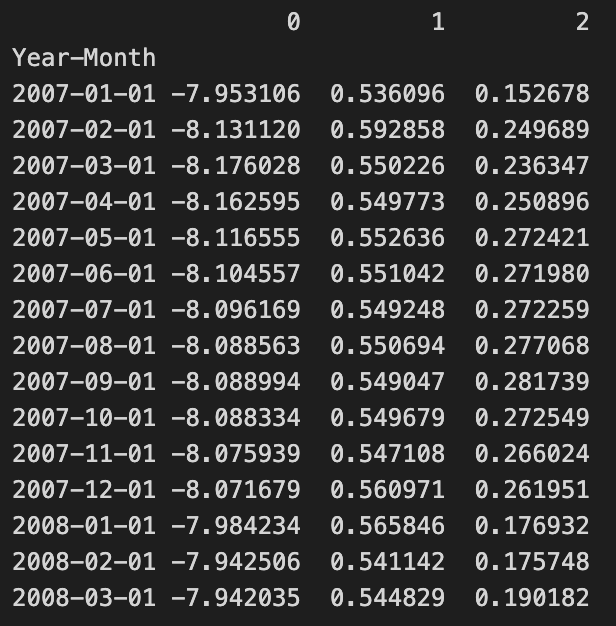
\includegraphics[width=0.5\linewidth]{PCA.png}
    \caption*{Dimension Reduced Dataset}
\end{figure}
which will be used in the following part of VAR model training.\\

In the part of VAR:\\
The goal of employing a VAR model was to capture the relationships and dynamics across the multiple time series represented by the principal components from PCA, thereby forecasting future values effectively.\\

We split the dataset into two parts, one is the train set used to train the model, another is the test set to evaluate the performance of the model.\\
After using the train set to train the model, we can get this outcome:
\begin{figure}[H]
    \centering
    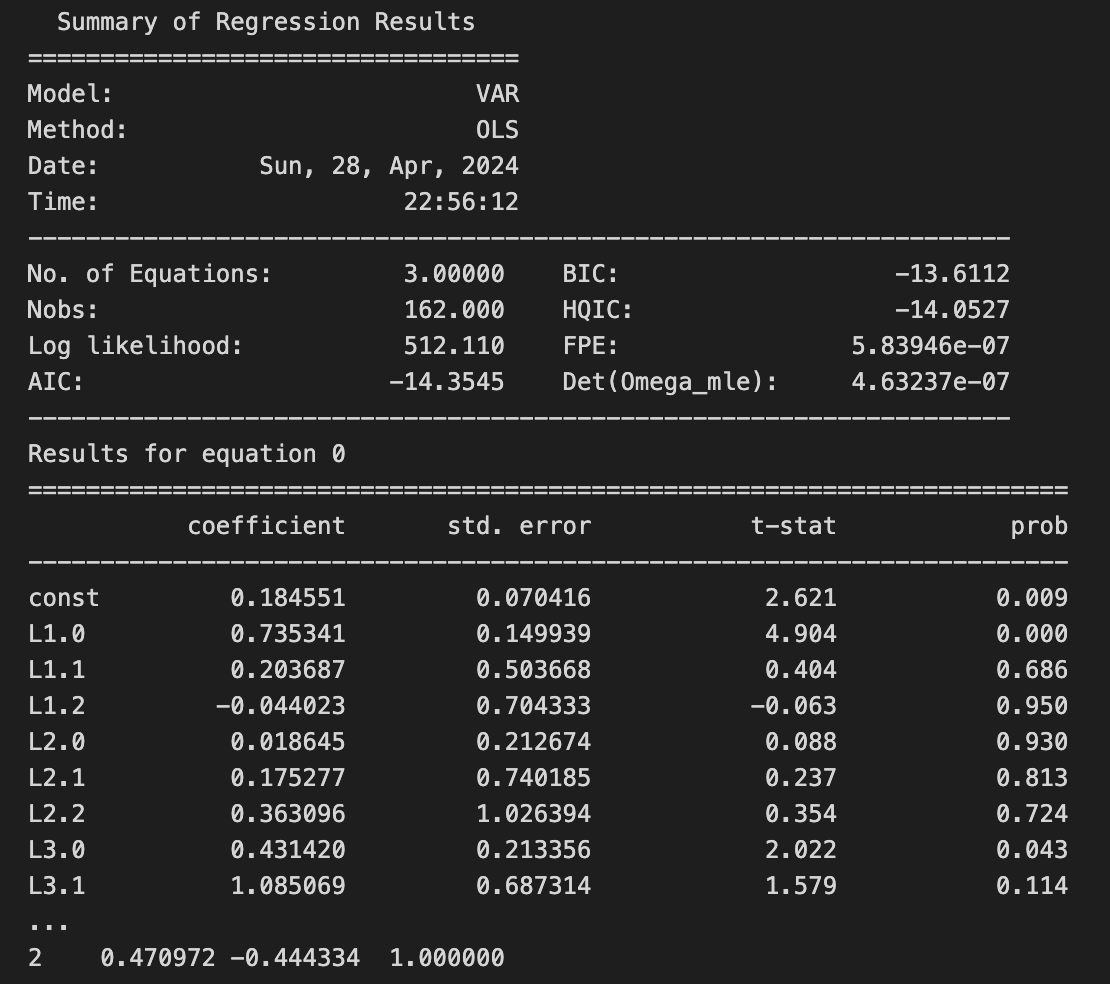
\includegraphics[width=0.5\linewidth]{VAR summary.png}
    \caption*{VAR Summary}
\end{figure}
However, we need to transform the principal components dataset back to the original dataset. After the transformation, we can get the predicted data like this:\\
\begin{figure}[H]
    \centering
    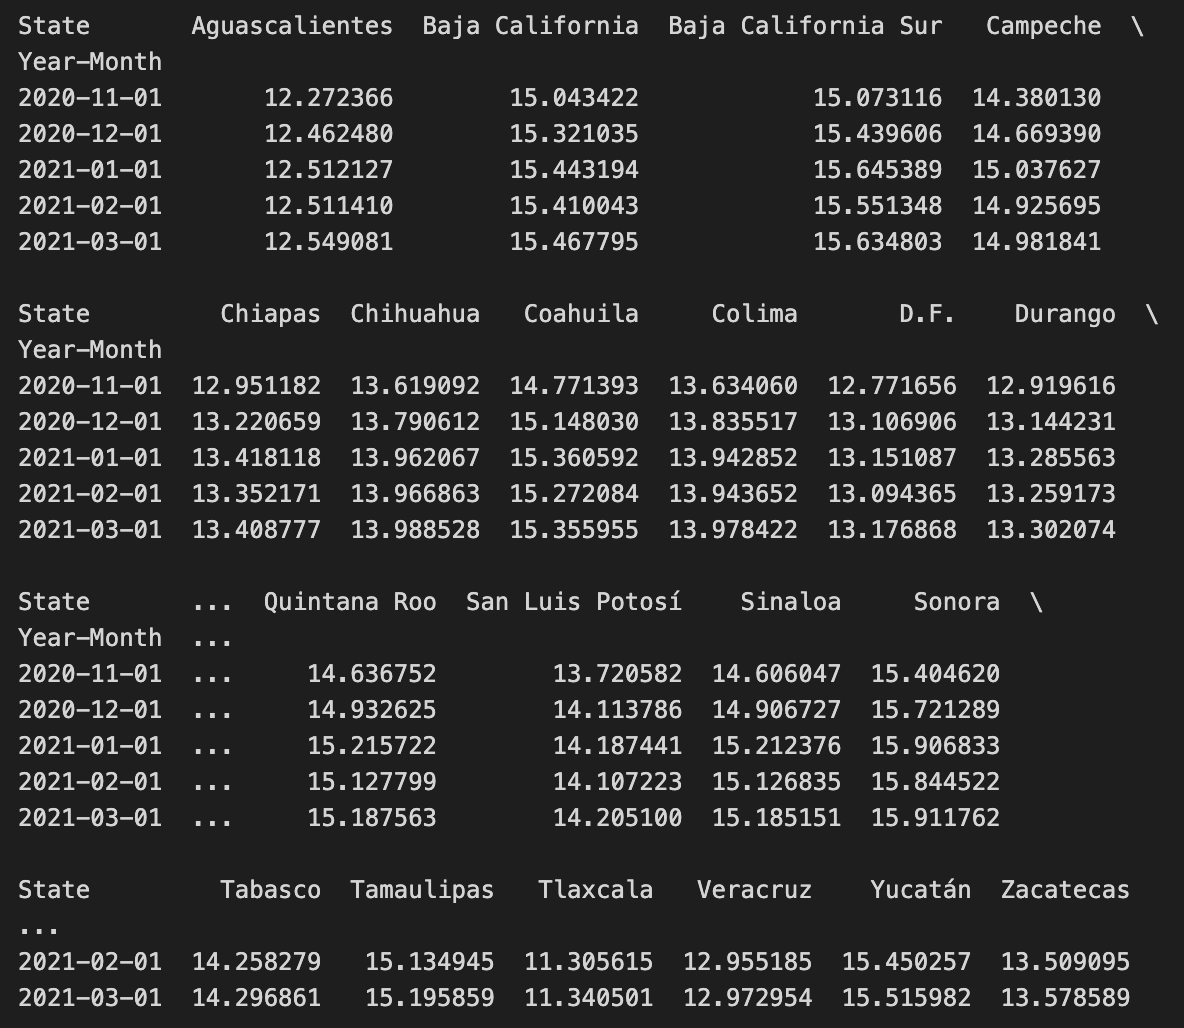
\includegraphics[width=0.5\linewidth]{Forecast.png}
    \caption*{Predicted Price per Kilogram}
\end{figure}
To evaluate the performance of this model, we can display the performance metrics, such as MAE, MSE and RMSE. The performance metrics are as following:
\begin{itemize}
    \item \textbf{MAE}: 2.743260393884601
    \item \textbf{MSE}: 10.399427076313355
    \item \textbf{RMSE}: 3.224814270049262
\end{itemize}

To evaluate the performance of the model, we can visualize the outcomes. Since there are so many states, we can select some important ones:\\
\begin{figure}[H]
    \centering
    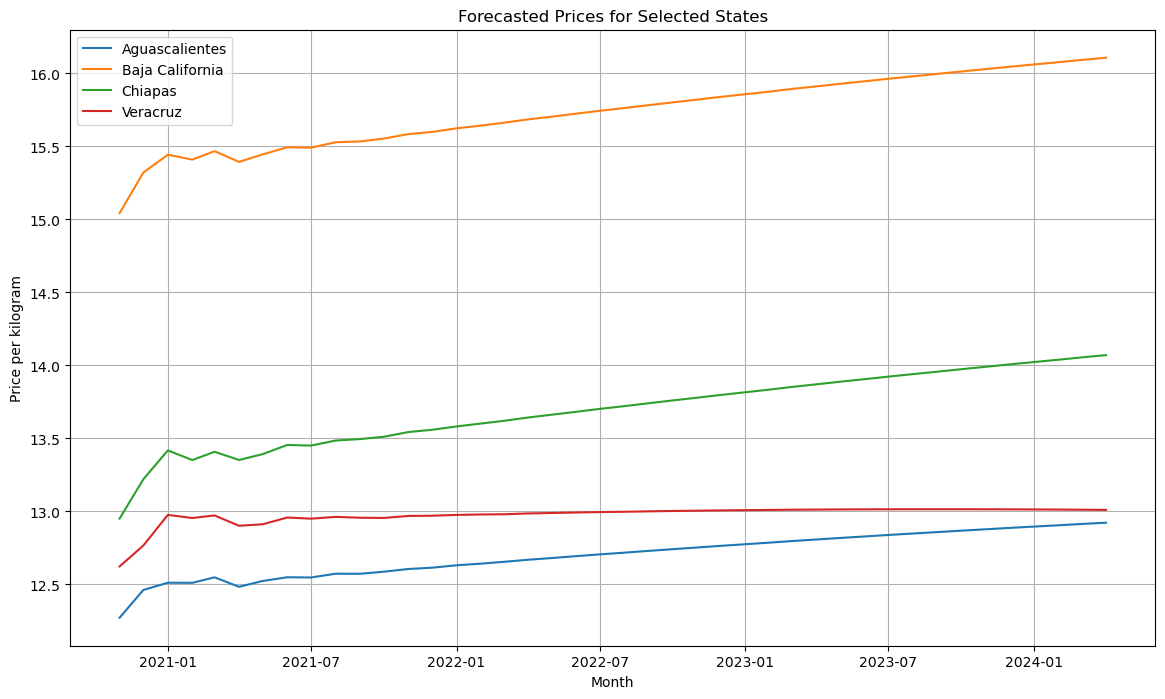
\includegraphics[width=1\linewidth]{Visualization for some states.png}
    \caption*{Predicted Prices for Selected States}
\end{figure}
To make a clearer evaluation, we can compare the predicted with the true values. 
\begin{figure}[H]
    \centering
    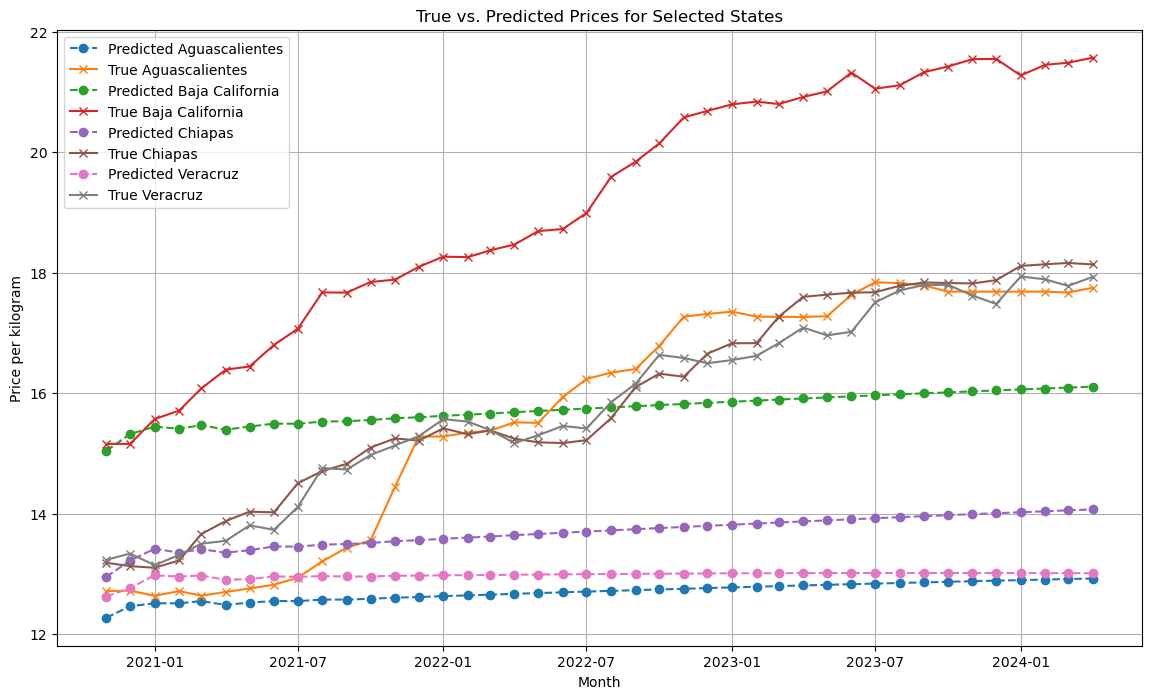
\includegraphics[width=1\linewidth]{Comparison.png}
    \caption*{Comparison between Predicted and True}
\end{figure}

\subsection*{4.Conclusion}
For the part of PCA, we successfully reduce the dimension from 32 to 3, is crucial for simplifying the modeling process without significantly compromising the data's integrity. Besides, the PCA retained 99\% of the variance with fewer components than the original number of states, which is significant for the training part.\\

In the part of VAR, we can make conclusions from two parts.\\
The first one is the performance matrix:\\
\textbf{Mean Absolute Error (MAE)}: The MAE of 2.743 means that, on average, the forecasted prices are approximately 2.743 units away from the actual prices. Given the units are in the price per kilogram, this deviation represents the average magnitude of errors in the predictions without considering their direction. An MAE closer to 0 indicates better performance. In economic terms, an MAE of this size might be considered acceptable, depending on the pricing scale and variability inherent to the dataset.\\

\textbf{Mean Squared Error (MSE)}: An MSE of 10.399 indicates the average squared difference between the estimated values and the actual value. The squaring of errors penalizes larger discrepancies more severely than smaller ones. A lower MSE is better, as it suggests less variability in the forecast errors. The relatively moderate MSE in our case suggests that while the model is generally reliable, there may be occasional forecasts that are significantly off from the true prices.\\

\textbf{Root Mean Squared Error (RMSE)}: The RMSE value of 3.225, being the square root of the MSE, is particularly informative as it returns the units to the original price per kilogram, making it directly interpretable. It suggests that most of the model's forecasts fall within approximately 3.225 units of the actual prices. This is beneficial for understanding the model's accuracy in the same units as the data.\\

To sum up, the performance metrics (MAE, MSE, RMSE) validate the visual observations, with the model achieving a reasonable degree of accuracy, which, while not perfect, provides a reliable basis for understanding price movements and making informed decisions.\\

The second one is the visualization:\\
Even though we think the model is of great accuracy from the performance matrix, we find it still need to be improved from the comparison.\\
From the comparison we obtain that the predicted ones closely track the actual ones. However, after 2021-1, the difference enlarges significantly, especially in the state of "Baja California".\\
Therefore, there are a lot needed to be improved: regularly updating the model with the latest data will help capture more recent trends, potentially improving the accuracy of forecasts. Besides, for areas where predictions diverge significantly from actual prices, a deeper analysis is recommended to uncover the reasons behind these discrepancies and to understand whether these are one-off events or part of a new trend.

\bibliography{bibliography}
\end{document}